\documentclass{article}
\usepackage{multicol}
\usepackage{hyperref}
\usepackage{footnote}
\usepackage{graphicx}
\usepackage{mathbbol}
\usepackage[bottom]{footmisc}

\graphicspath{ {./assets/} }

\title{Bezier Finance Whitepaper}
\author{Flydexo}

\begin{document}
\maketitle
\begin{abstract}
    DeFi is not easy to use for inexperienced or non-technical people. Content creators answered partly to this problem by creating videos or charts on Twitter with Excalidraw. The problem: Excalidraw isn't made for this, schemas are inconsistent so the terms and figures aren't always the same, strategies are not easily accessible and understandable, and last but not least the presented strategies are temporary but the schema is permanent.
    Bezier Finance is a web tool (SaaS) allowing users to visually create and share DeFi strategies. Each strategy is represented by a flowchart built with blocks and contains on-chain data updated every day. A strategy starts and ends with a wallet block. You can operate on liquidity flows to create a precise and custom strategy.
\end{abstract}
\pagebreak
\tableofcontents
\pagebreak
\section{Introduction}
Bezier Finance is a software as a service (SaaS) that started in October 2022. It was created to answer the main problem with decentralized finance currently: Accessibility. This problem discouraged users from using DeFi and instead they use centralized services increasing the risks of bankruptcy, reducing transparency, and ignoring blockchain and decentralization values.
\section{Integrations}
Bezier Finance is a multi-chain tool currently only supporting EVM-Compatible chains. To operate and provide a diversity of yields in the ecosystem Bezier is integrated with popular chains and protocols.
\subsection{Chains}
Bezier Finance supports 3 EVM compatible chains for the moment:
\begin{itemize}
    \item Ethereum
    \item Polygon
    \item Avalanche
\end{itemize}
Those chains support a variety of popular protocols, even some protocols are on the three chains.
\subsection{Protocols}
Bezier Finance supports 10 protocols:
\begin{itemize}
    \item Curve
    \item Uniswap V2
    \item Uniswap V3
    \item Aave V2
    \item Aave V3
    \item Beefy
    \item QiDAO / Mai Finance
    \item Lido
    \item Trader Joe
    \item Stake DAO
\end{itemize}
Those protocols provide a variety of yield methods and interactions. 
\label{sec:integration__yield}
\subsection{Yields}
On Bezier Finance a yield has inputs and outputs. Input is an asset type. An output has an asset type and a multiplier. This multiplier can be positive (e.g liquidity providing) or negative (e.g borrowing). A yield can have multiple inputs and outputs. Some inputs are optional and some outputs depend on the type of input. An input can have multiple outputs and the opposite. Let's take an example with the CRV liquid locker on Stake DAO\footnote{\url{https://lockers.stakedao.org/lockers/crv}}. This yield asks for input from either CRV or sdCRV \footnote{liquid locker CRV token}. And in output, you get 3CRV \footnote{Curve LP Token for the USDT-USDC-DAI pool}, CRV and SDT \footnote{Stake DAO governance token}.
\section{Use cases}
\subsection{Retail Investor}
In most cases, if you want to generate an interesting yield with DeFi you have to use different mechanisms and protocols. Bezier helps you to create strategies including multiple protocols to visually understand how to combine multiple protocols to optimize the yield.
\subsection{Content Creator}
Content creators on Twitter and YouTube for example can create strategies and share them with their community so they can understand better the why? and how? of the strategy.
\subsection{Education}
Many pieces of training exist to explain DeFi to the rookies and no tooling exists already to study and teach DeFi.
\subsection{CeFi transparency}
Even if DeFi will be getting simpler with time. People will still want to use centralized services because they don't want to manage their funds. But those users still need transparency about how the service generates yield. Bezier can be used for this purpose. 
\section{Tools}
Bezier Finance provides a complete toolset to create custom DeFi strategies. Bezier will represent the strategy's schema as a graph where each node is a tool (except Text, Image, Arrow) and has $n$ inputs $n$ outputs and a $x$ multiplier for each output.
\begin{center}
    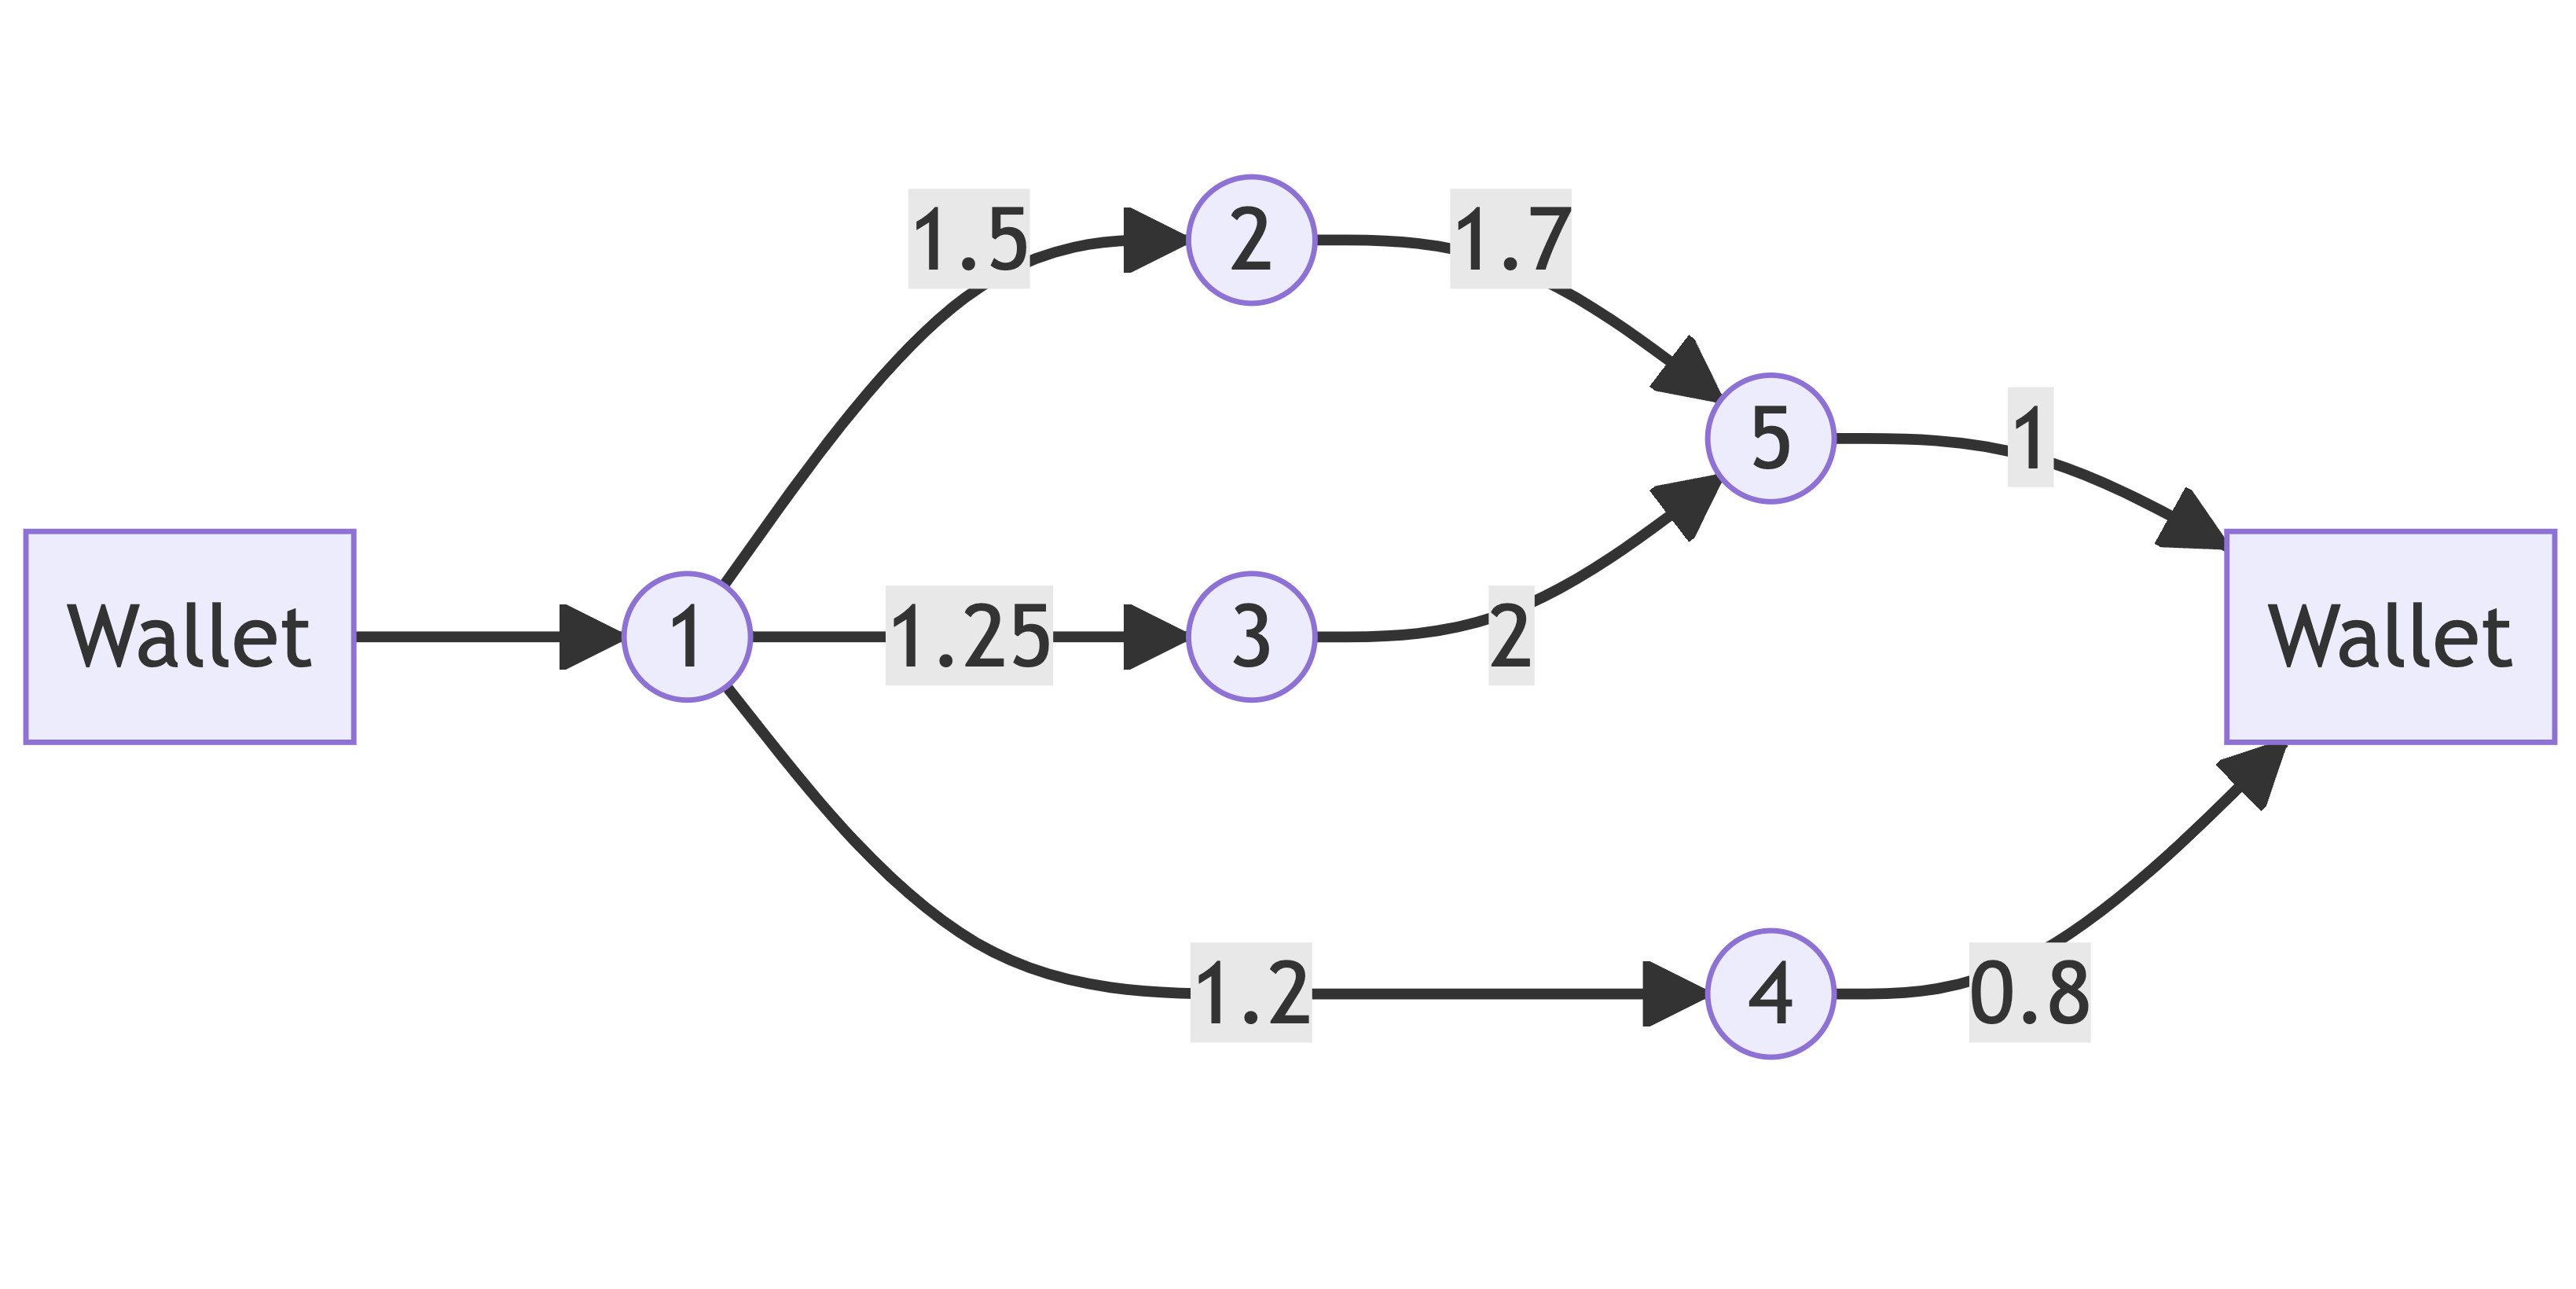
\includegraphics[scale=0.2]{graph.png}
\end{center}
\subsection{Wallet}
A wallet includes multiple assets and is used to compute the global strategy APY. For this purpose two wallets are necessary, the initial (before strategy) and the final (after strategy). If a flow isn't linked to the final wallet, it won't be accounted for in the final APY calculation. This also forces strategy creators to have their own reward token policy (swap and compound, farm and sell, hold).
\subsection{Yield}
The yield as described in the \hyperref[sec:integration__yield]{yields integration} has inputs and outputs with a multiplier. To compute the global APY, all yields inner a flow will count.
\subsection{Compound}
The compound tool sits on top of the yield tool. It increases the APY based on the number of times your compound the yield output in a year.
\subsection{Swap}
The swap tool transforms one token into another respecting the price ratio.
\subsection{Unwrapper}
The Unwrapper tool can wrap or unwrap a Liquidity Token to the underlying tokens or the opposite. (e.g 3CRV to DAI, USDC, USDT)
\subsection{Math}
The math tool operates simple calculus on a flow.
\subsubsection{Split}
The Split tool is a math tool that splits a flow of an asset to $n \in \mathbb{N}$ equal flows.
\subsubsection{Join}
The join tool is the opposite of the split tool, it outputs a single flow from multiple flows from the same asset.
\subsection{Arrow}
The arrow is the essential tool for Bezier, it represents the 'flow' mentioned earlier and links tools together. Has an origin and a destination.
\subsection{Image}
Shows an image on the canvas.
\subsection{Text}
Custom text on the canvas.
\section{Subscription plan}
The alpha release will only include a single subscription plan at 15\$/mo. When other plans will be added this plan will be the highest available plan. See \hyperref[sec:roadmap]{Roadmap}.
\section{Architecture}
\subsection{Frontend}
Our frontend is made with React\footnote{\url{https://reactjs.org}} and TypeScript\footnote{\url{https://typescriptlang.org}} and runs on Vercel\footnote{\url{https://vercel.com}}.
\subsection{Backend}
Every day, at 3 a.m. our on-chain scraper written in Golang queries on-chain, the graph\footnote{\url{https://thegraph.com/en/}} and API data. The data is then registered on our GitHub repo\footnote{\url{https://github.com/bezier-fi/data}} it is also replicated on our custom S3\footnote{Common protocol for storing files, JSON in our case, popular with AWS}.
\subsection{On-chain}
The current version of Bezier does not need on-chain computation, which will be needed for the 1 click strategy. See \hyperref[sec:roadmap]{Roadmap}.
\subsection{Payment}
Bezier will be using Superfluid\footnote{\url{https://www.superfluid.finance/}} to handle subscriptions, this allows the user to pay only for its usage of Bezier.
\pagebreak
\section{Roadmap}
\label{sec:roadmap}
\begin{multicols*}{2}
    \begin{itemize}
        \item [\textbf{Q1 2O23}]
        \item Launch alpha version
    \end{itemize}
    \begin{itemize}
        \item [\textbf{Q3 2O23}]
        \item Add more chains
        \subitem Arbitrum 
        \subitem Optimism
        \item Add more protocols
        \subitem Convex Finance
        \subitem Instadapp
        \subitem Compound
        \subitem Balancer
        \subitem Radiant
        \subitem Velodrome
    \end{itemize}
    \begin{itemize}
        \item [\textbf{Q1 2O24}]
        \item Social Portfolio
    \end{itemize}
    \vfill\null
    \columnbreak
    \begin{itemize}
        \item [\textbf{Q2 2O23}]
        \item Integrated social media with Lens Protocol
    \end{itemize}
    \begin{itemize}
        \item [\textbf{Q4 2O23}]
        \item apply strategy with one click
        \item from address to strategy
    \end{itemize}
\end{multicols*}
\end{document}